% arara: clean: {
% arara: --> extensions:
% arara: --> ['log','idx','ilg','ind','out','bbl','blg','thm','toc','aux','synctex.gz','bcf','run.xml','contb',
% arara: --> 'contg','contn','diffb','diffg','diffn','funb','fung','funn','genb','geng','genn','intb','intg','pytxcode',
% arara: --> 'intn','limb','limg','limn','logb','logg','logn','realb','realg','realn','seqb','seqg','seqn','ist',
% arara: --> 'serb','serg','sern','setb','setg','setn','ssfunb','ssfung','ssfunn','topb','topg','topn','pdf']
% arara: --> }
% arara: lualatex: {
% arara: --> shell: yes,
% arara: --> draft: yes,
% arara: --> }
% arara: biber
% arara: pythontex
% arara: lualatex: {
% arara: --> shell: yes,
% arara: --> draft: yes,
% arara: --> }
% arara: lualatex: {
% arara: --> shell: yes,
% arara: --> synctex: yes,
% arara: --> interaction: batchmode
% arara: --> }
% arara: clean: {
% arara: --> extensions:
% arara: --> ['log','idx','ilg','ind','out','bbl','blg','thm','toc','aux','bcf','run.xml','contb',
% arara: --> 'contg','contn','diffb','diffg','diffn','funb','fung','funn','genb','geng','genn','intb','intg','pytxcode',
% arara: --> 'intn','limb','limg','limn','logb','logg','logn','realb','realg','realn','seqb','seqg','seqn','ist',
% arara: --> 'serb','serg','sern','setb','setg','setn','ssfunb','ssfung','ssfunn','topb','topg','topn','nav','snm']
% arara: --> }
% !arara This a comment, hence works %%. Non-working in OpenJDK 13 :)
% arara: clean: {
% arara: --> extensions:
% arara: --> ['log','idx','ilg','ind','out','bbl','blg','thm','toc','aux','synctex.gz','bcf','run.xml','contb',
% arara: --> 'contg','contn','diffb','diffg','diffn','funb','fung','funn','genb','geng','genn','intb','intg','pytxcode',
% arara: --> 'intn','limb','limg','limn','logb','logg','logn','realb','realg','realn','seqb','seqg','seqn','ist',
% arara: --> 'serb','serg','sern','setb','setg','setn','ssfunb','ssfung','ssfunn','topb','topg','topn','pdf']
% arara: --> }
% arara: lualatex: {
% arara: --> shell: yes,
% arara: --> draft: yes,
% arara: --> }
% arara: biber
% arara: pythontex
% arara: lualatex: {
% arara: --> shell: yes,
% arara: --> draft: yes,
% arara: --> }
% arara: lualatex: {
% arara: --> shell: yes,
% arara: --> synctex: yes,
% arara: --> interaction: batchmode
% arara: --> }
% arara: clean: {
% arara: --> extensions:
% arara: --> ['log','idx','ilg','ind','out','bbl','blg','thm','toc','aux','bcf','run.xml','contb',
% arara: --> 'contg','contn','diffb','diffg','diffn','funb','fung','funn','genb','geng','genn','intb','intg','pytxcode',
% arara: --> 'intn','limb','limg','limn','logb','logg','logn','realb','realg','realn','seqb','seqg','seqn','ist',
% arara: --> 'serb','serg','sern','setb','setg','setn','ssfunb','ssfung','ssfunn','topb','topg','topn','nav','snm']
% arara: --> }
% !arara This a comment, hence works %%. Non-working in OpenJDK 13 :)
% arara: clean: {
% arara: --> extensions:
% arara: --> ['log','idx','ilg','ind','out','bbl','blg','thm','toc','aux','synctex.gz','bcf','run.xml','contb',
% arara: --> 'contg','contn','diffb','diffg','diffn','funb','fung','funn','genb','geng','genn','intb','intg','pytxcode',
% arara: --> 'intn','limb','limg','limn','logb','logg','logn','realb','realg','realn','seqb','seqg','seqn','ist',
% arara: --> 'serb','serg','sern','setb','setg','setn','ssfunb','ssfung','ssfunn','topb','topg','topn','pdf']
% arara: --> }
% arara: lualatex: {
% arara: --> shell: yes,
% arara: --> draft: yes,
% arara: --> }
% arara: biber
% arara: pythontex
% arara: lualatex: {
% arara: --> shell: yes,
% arara: --> draft: yes,
% arara: --> }
% arara: lualatex: {
% arara: --> shell: yes,
% arara: --> synctex: yes,
% arara: --> interaction: batchmode
% arara: --> }
% arara: clean: {
% arara: --> extensions:
% arara: --> ['log','idx','ilg','ind','out','bbl','blg','thm','toc','aux','bcf','run.xml','contb',
% arara: --> 'contg','contn','diffb','diffg','diffn','funb','fung','funn','genb','geng','genn','intb','intg','pytxcode',
% arara: --> 'intn','limb','limg','limn','logb','logg','logn','realb','realg','realn','seqb','seqg','seqn','ist',
% arara: --> 'serb','serg','sern','setb','setg','setn','ssfunb','ssfung','ssfunn','topb','topg','topn','nav','snm']
% arara: --> }
% !arara This a comment, hence works %%. Non-working in OpenJDK 13 :)
% arara: clean: {
% arara: --> extensions:
% arara: --> ['log','idx','ilg','ind','out','bbl','blg','thm','toc','aux','synctex.gz','bcf','run.xml','contb',
% arara: --> 'contg','contn','diffb','diffg','diffn','funb','fung','funn','genb','geng','genn','intb','intg','pytxcode',
% arara: --> 'intn','limb','limg','limn','logb','logg','logn','realb','realg','realn','seqb','seqg','seqn','ist',
% arara: --> 'serb','serg','sern','setb','setg','setn','ssfunb','ssfung','ssfunn','topb','topg','topn','pdf']
% arara: --> }
% arara: lualatex: {
% arara: --> shell: yes,
% arara: --> draft: yes,
% arara: --> }
% arara: biber
% arara: pythontex
% arara: lualatex: {
% arara: --> shell: yes,
% arara: --> draft: yes,
% arara: --> }
% arara: lualatex: {
% arara: --> shell: yes,
% arara: --> synctex: yes,
% arara: --> interaction: batchmode
% arara: --> }
% arara: clean: {
% arara: --> extensions:
% arara: --> ['log','idx','ilg','ind','out','bbl','blg','thm','toc','aux','bcf','run.xml','contb',
% arara: --> 'contg','contn','diffb','diffg','diffn','funb','fung','funn','genb','geng','genn','intb','intg','pytxcode',
% arara: --> 'intn','limb','limg','limn','logb','logg','logn','realb','realg','realn','seqb','seqg','seqn','ist',
% arara: --> 'serb','serg','sern','setb','setg','setn','ssfunb','ssfung','ssfunn','topb','topg','topn','nav','snm']
% arara: --> }
% !arara This a comment, hence works %%. Non-working in OpenJDK 13 :)
\input{beamer.tex.preamble}
\begin{document}

\include{./contents/introduction}
\include{./contents/models}
\include{./contents/references}

\end{document}
\begin{document}

\section{Introducción}

Este proyecto hace referencia a la función de producción de Cobb-Douglas, siendo este publicado en \cite{Douglas1976} 1928 por \citeauthor{Douglas1976}, quienes realizaron un estudio en el que se modeló el crecimiento de la economía estadounidense. Para este proyecto se desarrollará una aplicación con una base de datos como un caso particular, pero previo a su aplicación, se realizará una posible forma de cómo Charles Cobb y Paul Douglas llegaron a la formulación algebraica de la función. Al finalizar, se comparará la solución exacta de la ecuación con la obtenida por el método de mínimos cuadrados.

\subsection{Función de producción de Cobb-Douglas}

Para el análisis matemático de la función, es necesario describir los factores involucrados en el modelo.

\subsection{Función de producción}

Es la relación entre las cantidades máximas de productos que una empresa puede fabricar mediante el uso de diversas cantidades de insumos. Las múltiples funciones de producción están representadas por la combinación de factores de insumo (tecnología, capital, trabajo entre otros). Una función de producción se expresa como la ecuación~\eqref{eq:production} siguiente:
\begin{equation}\label{eq:production}
P=f(K,L,I)
\end{equation}
donde:
\begin{itemize}
	\item $P$ es la cantidad de producción.
	\item $K,L,I$ son los insumos.
\end{itemize}

\section{El proyecto}

En esta sección explicaré los detalles de mi proyecto y su visión. Espero que esta estructura se mejore considerablemente bajo la guía de mi mentor.

\subsection{Cobb-Douglas y la función de producción ACMS}

Partiendo de la función Cobb-Douglas
\begin{equation}%\label{eq:1}
Y = bL^{k}C^{1-k},
\end{equation}
donde:
\begin{itemize}
	\item $b$ representa el factor total de productividad,
	\item $Y$ la producción total,
	\item $L$ el trabajo,
	\item $C$ el capital.
\end{itemize}
Esta función fue generalizada siendo expresada de la manera siguiente:
\begin{equation}%\label{eq:2}
f = \gamma{x}_{1}^{\alpha_{1}}\cdots x_{n}^{\alpha_{n}},
\end{equation}
donde $\gamma$ es una constante positiva y $\alpha_{1},\ldots,\alpha_{n}$ son constantes no cero.

Se dice que una función de producción $f$ es $d$--homogénea o homogénea de degradación $d$, si:
\begin{equation}%\label{eq:3}
f\left(tx_{1},\ldots,tx_{n}\right) = t^{d}f\left(x_{1},\ldots,x_{n}\right),
\end{equation}
Se mantiene para cada $t\in\mathbb{R}$ en la función previamente definida.

Una función \emph{homogénea de degradación uno} es llamado como \emph{linealmente homogéneo}.

Si $d>1$, la función homogénea mostrará un crecimiento a escala, caso contrario cuando $d<1$ mostrará un decrecimiento a escala.

Arrow, Chenery, Minhas y Solow(ACMS) introdujeron una función de producción de dos factores:
\begin{equation}%\label{eq:4}
Q=F\cdot(aK^r + (1-a)L^r)^{1/r},
\end{equation}
donde:
\begin{itemize}
	\item $Q$ representa el resultado,
	\item $F$ el factor de producción,
	\item $a$ el parámetro compartido,
	\item $k,L$ los factores de producción primario,
	\item $r=\left(s-1\right)/s$ , $s=1/\left(1-r\right)$ como la substitución de elasticidad.
\end{itemize}

La función de producción generalizada de ACMS se define:
\begin{equation}\label{eq:5}
f\left(x\right) = \gamma\sum_{i=1}^{n} ({{a}_{i}^{p}x_{i}^{p}})^{d/p},x=\left(x_{1},\ldots,x_{n}\right)\in D\subset\mathbb{R}_{+}^{n},
\end{equation}
con $a_{1},\ldots,a_{n},\gamma,p\neq0$, donde $d$ es la degradación de homogeneidad.

Cabe resaltar que la \emph{función de producción homotética} tiene la siguiente expresión como una función de producción:
\begin{equation}\label{eq:6}
f(x) = F\left(h(x_1,\ldots,x_n\right),
\end{equation}
donde F es una función estrictamente creciente y $h\left(x_1,\ldots,x_n\right)$ es una función homogénea de cualquier degradación d. La \emph{función de producción homotética} de la forma:
\begin{equation}\label{eq:7}
f\left(x\right) = \gamma\sum_{i=1}^{n} ({{a}_{i}^{p}x_{i}^{p}})^{d/p},\quad(\text{resp.},\quad f(x)=F(x_{1}^{\alpha_1}\cdots x_{n}^{\alpha_n}),
\end{equation}
es llamada \emph{función de producción ACMS generalizada homotética}.

\subsection{Breve descripción}

Si $f$ es una función de dos variables, a menudo dejamos que una letra como $z$ denote el valor de $f$ en el punto $\left(x,y\right)$, así $z=f\left(x,y\right)$. Entonces llamaremos a $x$ e $y$ las \emph{variables independientes}, o los \emph{argumentos} de $f$, mientras que $z$ es llamada la \emph{variable independiente}, porque el valor $z$, en general, depende de los valores $x$ e $y$. El dominio de la función $f$ es entonces el conjunto de todos los posibles pares de variables independientes, mientras que su \emph{rango} es el conjunto de valores correspondientes de la variable dependientes. En economía, $x$ e $y$ son llamadas las variables \emph{exógenas}, mientras que $z$ es la variable \emph{endógena}.

Una función de dos variables que aparecen en muchos modelos económicos es
\begin{equation}\label{eq:cobb-douglas}
F\left(x,y\right)=Ax^{a}y^{b}
\end{equation}
donde $A$, $a$ y $b$ son constantes. Usualmente, uno asume que $F$ es definida solo para $x>0$ e $y>0$.

A función de la forma~\eqref{eq:cobb-douglas} es generalmente llamada la \emph{función de Coubb-Douglas}. Se usa con mayor frecuencia para describir ciertos procesos de producción. Entonces $x$ e $y$ son llamados \emph{factores de entrada}, mientras que $F\left(x,y\right)$ es el número de unidades producidas, o la \emph{salida}. En este caso $F$ es llamada la \emph{función de producción}.

%\subsubsection{Defining \pygment{python}{ImageSet} Union for Trigonometric Equation Solver}%\protect||

% TODO: Page 276.
\begin{example}[Elasticidad de sustitución constante]
	Considere la ``elasticidad de sustitución constante'', o la función \textsc{CES}
	\begin{equation}
	F\left(K,L\right)=A\left(aK^{-\rho}+\left(1-a\right)L^{-\rho}\right)^{-1/\rho}
	\end{equation}
	donde $A>0$, $K>0$, $L>0$, $a\in\left(0,1\right)$, y $\rho\neq 0$. Manteniendo $A,K,L$ y $a$ fijos, aplique la regla de L'H\^{o}pital a $z=\ln\left[F\left(K,L\right)/A\right]$  cuando $\rho\to0$ con el fin de mostrar que $F\left(K,L\right)$ converge a la función de Cobb-Douglas $AK^{a}L^{1-a}$.
\end{example}

\begin{proof}[Solución]
	Obtenemos \[ z=\ln{\left(aK^{-\rho}+\left(1-a\right)L^{-\rho}\right)}^{-1/\rho}=-\ln\left(aK^{-\rho}+\left(1-a\right)L^{-\rho}\right)/\rho\to\frac{0}{0}\text{ cuando }\rho\to0. \] Ya que $\left(\mathrm{d}/\mathrm{d}\rho\right)K^{-\rho}=-K^{-\rho}\ln K$ y $\left(\mathrm{d}/\mathrm{d}\rho\right)L^{-\rho}=-L^{-\rho}\ln L$, aplicando la regla de L'H\^{o}pital da
	\begin{align*}
	\lim_{\rho\to0}z
	&=\lim_{\rho\to0}\left[\frac{aK^{-\rho}\ln K + \left(1-a\right)L^{-\rho}\ln L}{aK^{-\rho}+\left(1-a\right)L^{-\rho}}\right]\\
	&=a\ln K+\left(1-a\right)\ln L\\
	&=\ln K^{a}L^{1-a}.
	\end{align*}
	Por lo tanto, $e^{z}\to K^{a}L^{1-a}$. De la definición de $z$, se sigue que $F\left(K,L\right)\to AK^{a}L^{1-a}$ cuando $\rho\to0$.
\end{proof}

%pag. 408-409
\begin{example}[Función de Cobb-Douglas]
	Una función de dos variables que aparece en muchos modelos económicos es
	\begin{equation}\label{eq:cobb}
	F\left(x,y\right)=Ax^{a}y^{b}
	\end{equation}
	donde $A$, $a$ y $b$b son constantes. Usualmente, uno asume que $F$ está definida sola pora $x>0$ e $y>0$.

	Una función $F$ de la forma~\eqref{eq:cobb} es generalmente llamada la \emph{función de Cobb-Douglas}\footnote{La función en~\eqref{eq:cobb} es llamada en honor a los investigadores americanos C.W.Cobb y P.H.Douglas, quien aplicaron esto, con  $a+b=1$, en un articulo científico que aparecio en 1927 en la estimacion de una función de producción. Sin embargo, deberia correctamente ser llamada la ``función de Wicksell'', porque el economista sueco K.Wicksell(1851-1926) introdujo tales funciones de producción antes de 1900.}. Con frecuencia es usada para describir ciertos procesos productivos. Así, $x$ e $y$ son llamados los \emph{factores de entrada}, mientras que $F\left(x,y\right)$ es el número de unidades producidas, o la \emph{salida}. En este caso, $F$ es llamada una \emph{función de producción}.
\end{example}

\begin{example}
	Suponga que $F\left(K,L\right)$ modela la producción de una empresa cuando sus entradas son capital y labor, respectivamente $K$ y $L$. Una curva de nivel por esta función de producción es una curva en el plano $KL$ dado por $F\left(K,L\right)=Y_{o}$, donde $Y_{0}$ es una constante. Esta curva es llamada una \emph{isocuanta}, que significa ``igual cantidad''. Para una función de Cobb-Douglas, $F\left(K,L\right)=AK^{a}L^{b}$, con $a+b<1$ y $A>0$, las figuras~\ref{fig:1} y~\ref{fig:2}, respectivamente, muestra una parte de la gráfica cerca del origen, y tres de las isocuantas.
	
	\begin{figure}[ht!]
		\begin{minipage}[c]{0.4\linewidth}
			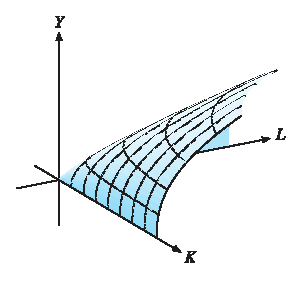
\includegraphics[width=\linewidth]{figure1}\label{fig:1}
			\caption{Gráfica de la función de producción Cobb-Douglas.}
		\end{minipage}
		\hfill
		\begin{minipage}[c]{0.4\linewidth}
			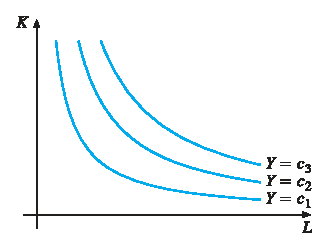
\includegraphics[width=\linewidth]{figure2}\label{fig:2}
			\caption{Isocuantas de la función de producción Cobb-Douglas.}
		\end{minipage}
	\end{figure}
\end{example}
% pag. 428
\begin{example}[Funciones $n$--lineales y $\log$--lineales]
	\leavevmode
	\begin{enumerate}
		\item\label{item:a} La demanda del azúcar en los Estados Unidos durante el período 1929--1936 fue estimado para ser descrito, aproximadamente, por la fórmula \[ x=108.83-6.0294p+0.164w-0.4217t \] donde $x$ es la demanda del azúcar, $p$ es su precio, $w$ es un índice de producción y $t$ es el año (donde $t=0$ corresponde a 1929).
		\item\label{item:b} La siguiente fórmula es una estimación para la demanda de cerveza en el Reino Unido: \[ x=1.058{x}^{0.136}_{1}{x}^{-0.727}_{2}{x}^{0.914}_{3}x^{0.816}_{4}. \]
		Aquí la cantidad demandada, $x$, es una función de cuatro variables: $x_{1}$, el ingreso per cápita, $x_{2}$, el precio de la cerveza, $x_{3}$, índice general de precios de productos básicos y $x_{4}$, la fuerza de la cerveza.
	\end{enumerate}
\end{example}
Las funciones más simples en el ejemplo anterior es la única en la parte~\eqref{item:a}. Las variables $p$, $w$ y $t$ ocurren solo cuando a la primera potencia, y ellas son multiplicadas por constantes, no por cada otra. Tales funciones son llamadas \emph{lineales}. En general
\begin{equation}
f\left(x_{1},x_{2},\ldots,x_{n}\right)=a_{1}x_{1}+a_{2}x_{2}+\cdots+a_{n}x_{n}+b
\end{equation}
donde $a_{1},a_{2},\ldots,a_{n}$ y $b$ son constantes, es una \emph{función lineal} en $n$ variables.

La función en la parte~\eqref{item:b} del ejemplo  es un caso especial de la función general de Cobb-Douglas
\begin{equation}\label{eq:cobbgeneralized}
F\left(x_{1},x_{2},\ldots,x_{3}\right)=A{x}^{a_{1}}_{1}{x}^{a_{2}}_{2}\cdots{x}^{a_{n}}_{n}
\end{equation}
donde $A>0$, $a_{1},\ldots,a_{n}$ son constantes, definidas para $x_{1}>0,x_{2}>0,\ldots x_{n}>0$. Note que al tomar el logaritmo natural a cada lado de~\eqref{eq:cobbgeneralized} resulta
\begin{equation}
\ln F=\ln A+a_{1}\ln x_{1}+a_{2}\ln x_{2}+\cdots+a_{n}\ln x_{n}.
\end{equation}
Esto muestra que la función de Cobb-Douglas es $\log$--lineal, ya que $\ln F$ es una función lineal para $\ln x_{1},\ln x_{2},\ldots,\ln x_{n}$.
\subsection{Modelo de crecimiento de Solow}
\begin{example}[Modelo de crecimiento de Solow]
Este modelo de crecimiento neoclásico está basado en la ecuación diferencial
\begin{equation}\label{eq:solowgrowth}
\dot{k}=sf\left(k\right)-\lambda k
\end{equation}
Aquí la función desconocida $k=k(t)$ denota el capital por trabajador, $s>0$ denota la tasa constante de ahorro, $f$ es una función de producción (producto nacional por trabajador como una función del capital por trabajador), y $\lambda>0$ denota la tasa proporcional constante de crecimiento del número de trabajadores.
\end{example}

Note que~\eqref{eq:solowgrowth} es una ecuacion separable. Debido a que $f$ no se especifica, aún no podemos encontrar una solución explícita de la ecuación. Asuma que el diagrama de fase para la ecuación~\eqref{eq:solowgrowth} es como se muestra en la Fig.4. % TODO: Incluir figura 4.
Luego, aquí un estado de equilibrio único con $k^{\ast}>0$. Esto es dado por:
\begin{equation}
sf\left(k^{\ast}\right)=\lambda k^{\ast}
\end{equation}
Por inspección de la Fig.4 vemos que $k^{\ast}$ es estable. Sin importar cuál ha sido el capital inicial por trabajador $k\left(0\right)$, $k\left(t\right)\rightarrow k^{\ast}$ cuando $t\rightarrow\infty$.

% (pag. 212)
%\caption{Diagrama de fase para~\eqref{eq:solowgrowth}, con condicion apropiada en $f$.}

Este es ua modelo mas detallado que lleva a la ecuación ~\eqref{eq:solowgrowth}. Sea $X\left(t\right)$ que denota el ingreso nacional, $K\left(t\right)$ el capital, y
$L\left(t\right)$ el número de trabajadores en un país en un tiempo $t$. Asuma que
\begin{multicols}{3}
\begin{itemize}
	\item $X\left(t\right)=F\left(K(t),L(t)\right)$
	\item $\dot{K}\left(t\right)=sX\left(t\right)$
	\item $L\left(t\right)=L_{0}e^{\lambda t}$
\end{itemize}
\end{multicols}
donde $F$ es una función de producción, y $s$ es la tasa de ahorro. Asuma que $F$ es homogénea de grado $1$, así que $F\left(K,L\right)=LF\left(K/L,1\right)$ para todo $K$ y $L$.
Defina $k\left(t\right) =K\left(t\right)/L\left(t\right)=$ capital por trabajador, y $f\left(k\right)=F\left(k,1\right)=F\left(K/L,1\right)=F\left(K,L\right)/L=$ salida por trabajador. Luego,  $\dot{k}/k=\left(d/dt\right)\left(\ln k\right)=\left(d/dt\right)\left(\ln K-\ln L\right)$, y así
\begin{equation}
\frac{\dot{k}}{k}=\frac{\dot{K}}{K}-\dfrac{\dot{L}}{L}=\frac{sF\left(K,L\right)}{K}-\lambda=\frac{sLf\left(k\right)}{K}-\lambda=\frac{sf\left(k\right)}{k}-\lambda
\end{equation}
de la cual~\eqref{eq:solowgrowth} sigue a la vez.

\begin{remark}
	Déjenes discutir brevemente las condciones suficientes para la existencia y unicidad del equilibrio del modelo de Solow. Es usual asumir que $f\left(0\right)=0$, así como que $f^{\prime}\left(k\right)>0$ y $f^{\prime\prime}\left(k\right)<0$ para todo $k>0$. Esto es también común postular las llamadas \emph{condiciones de Inada}, de acuerdo con $f^{\prime}\left(k\right)\rightarrow\infty$ y también $f^{\prime}\left(k\right)\rightarrow0$ cuando $k\rightarrow\infty$.
	
	Para ver por qué estas condiciones son suficientes, defina $G\left(k\right)=sf\left(k\right)-\lambda k$. Entonces, $G^{\prime}\left(k\right)=sf^{\prime}\left(k\right)-\lambda$, y la ecuación~\eqref{eq:solowgrowth} cambia a $\dot{k}=G\left(k\right)$. Los supuestos sobre $f$ implica que $G\left(0\right)=0$, $G^{\prime}\left(k\right)\rightarrow\infty$ cuando $k\rightarrow0$, $G^{\prime}\left(k\right)\rightarrow-\lambda<0$ cuando $k\rightarrow\infty$, y $G^{\prime\prime}\left(k\right)=sf^{\prime\prime}\left(k\right)<0$ para todo $k>0$. Así $G$ tiene un único punto estacionario $\hat{k}>0$ en el cual $G^{\prime}\left(\hat{k}\right)=0$. Obviamente, $G\left(\hat{k}\right)>0$. Pero, $G^{\prime}\left(k\right)<-\frac{1}{2}\lambda<0$ para cualquier $k$ suficientemente grande. Se sigue que $G\left(k\right)\rightarrow-\infty$ cuando $k\rightarrow\infty$, así que existe un único punto $k^{\ast}>0$ con $G\left(k^{\ast}\right)=0$. Adicionalmente, $G^{\prime}\left(k^{\ast}\right)<0$. De acuerdo con % TODO
	esta es una condición suficiente para la estabilidad local asintótica de $k^{\ast}$.
\end{remark}
\nocite{*}
\printbibliography[title={Referencias bibliográficas},heading=bibintoc]

\end{document}
\begin{document}

\section{Introducción}

Este proyecto hace referencia a la función de producción de Cobb-Douglas, siendo este publicado en \cite{Douglas1976} 1928 por \citeauthor{Douglas1976}, quienes realizaron un estudio en el que se modeló el crecimiento de la economía estadounidense. Para este proyecto se desarrollará una aplicación con una base de datos como un caso particular, pero previo a su aplicación, se realizará una posible forma de cómo Charles Cobb y Paul Douglas llegaron a la formulación algebraica de la función. Al finalizar, se comparará la solución exacta de la ecuación con la obtenida por el método de mínimos cuadrados.

\subsection{Función de producción de Cobb-Douglas}

Para el análisis matemático de la función, es necesario describir los factores involucrados en el modelo.

\subsection{Función de producción}

Es la relación entre las cantidades máximas de productos que una empresa puede fabricar mediante el uso de diversas cantidades de insumos. Las múltiples funciones de producción están representadas por la combinación de factores de insumo (tecnología, capital, trabajo entre otros). Una función de producción se expresa como la ecuación~\eqref{eq:production} siguiente:
\begin{equation}\label{eq:production}
P=f(K,L,I)
\end{equation}
donde:
\begin{itemize}
	\item $P$ es la cantidad de producción.
	\item $K,L,I$ son los insumos.
\end{itemize}

\section{El proyecto}

En esta sección explicaré los detalles de mi proyecto y su visión. Espero que esta estructura se mejore considerablemente bajo la guía de mi mentor.

\subsection{Cobb-Douglas y la función de producción ACMS}

Partiendo de la función Cobb-Douglas
\begin{equation}%\label{eq:1}
Y = bL^{k}C^{1-k},
\end{equation}
donde:
\begin{itemize}
	\item $b$ representa el factor total de productividad,
	\item $Y$ la producción total,
	\item $L$ el trabajo,
	\item $C$ el capital.
\end{itemize}
Esta función fue generalizada siendo expresada de la manera siguiente:
\begin{equation}%\label{eq:2}
f = \gamma{x}_{1}^{\alpha_{1}}\cdots x_{n}^{\alpha_{n}},
\end{equation}
donde $\gamma$ es una constante positiva y $\alpha_{1},\ldots,\alpha_{n}$ son constantes no cero.

Se dice que una función de producción $f$ es $d$--homogénea o homogénea de degradación $d$, si:
\begin{equation}%\label{eq:3}
f\left(tx_{1},\ldots,tx_{n}\right) = t^{d}f\left(x_{1},\ldots,x_{n}\right),
\end{equation}
Se mantiene para cada $t\in\mathbb{R}$ en la función previamente definida.

Una función \emph{homogénea de degradación uno} es llamado como \emph{linealmente homogéneo}.

Si $d>1$, la función homogénea mostrará un crecimiento a escala, caso contrario cuando $d<1$ mostrará un decrecimiento a escala.

Arrow, Chenery, Minhas y Solow(ACMS) introdujeron una función de producción de dos factores:
\begin{equation}%\label{eq:4}
Q=F\cdot(aK^r + (1-a)L^r)^{1/r},
\end{equation}
donde:
\begin{itemize}
	\item $Q$ representa el resultado,
	\item $F$ el factor de producción,
	\item $a$ el parámetro compartido,
	\item $k,L$ los factores de producción primario,
	\item $r=\left(s-1\right)/s$ , $s=1/\left(1-r\right)$ como la substitución de elasticidad.
\end{itemize}

La función de producción generalizada de ACMS se define:
\begin{equation}\label{eq:5}
f\left(x\right) = \gamma\sum_{i=1}^{n} ({{a}_{i}^{p}x_{i}^{p}})^{d/p},x=\left(x_{1},\ldots,x_{n}\right)\in D\subset\mathbb{R}_{+}^{n},
\end{equation}
con $a_{1},\ldots,a_{n},\gamma,p\neq0$, donde $d$ es la degradación de homogeneidad.

Cabe resaltar que la \emph{función de producción homotética} tiene la siguiente expresión como una función de producción:
\begin{equation}\label{eq:6}
f(x) = F\left(h(x_1,\ldots,x_n\right),
\end{equation}
donde F es una función estrictamente creciente y $h\left(x_1,\ldots,x_n\right)$ es una función homogénea de cualquier degradación d. La \emph{función de producción homotética} de la forma:
\begin{equation}\label{eq:7}
f\left(x\right) = \gamma\sum_{i=1}^{n} ({{a}_{i}^{p}x_{i}^{p}})^{d/p},\quad(\text{resp.},\quad f(x)=F(x_{1}^{\alpha_1}\cdots x_{n}^{\alpha_n}),
\end{equation}
es llamada \emph{función de producción ACMS generalizada homotética}.

\subsection{Breve descripción}

Si $f$ es una función de dos variables, a menudo dejamos que una letra como $z$ denote el valor de $f$ en el punto $\left(x,y\right)$, así $z=f\left(x,y\right)$. Entonces llamaremos a $x$ e $y$ las \emph{variables independientes}, o los \emph{argumentos} de $f$, mientras que $z$ es llamada la \emph{variable independiente}, porque el valor $z$, en general, depende de los valores $x$ e $y$. El dominio de la función $f$ es entonces el conjunto de todos los posibles pares de variables independientes, mientras que su \emph{rango} es el conjunto de valores correspondientes de la variable dependientes. En economía, $x$ e $y$ son llamadas las variables \emph{exógenas}, mientras que $z$ es la variable \emph{endógena}.

Una función de dos variables que aparecen en muchos modelos económicos es
\begin{equation}\label{eq:cobb-douglas}
F\left(x,y\right)=Ax^{a}y^{b}
\end{equation}
donde $A$, $a$ y $b$ son constantes. Usualmente, uno asume que $F$ es definida solo para $x>0$ e $y>0$.

A función de la forma~\eqref{eq:cobb-douglas} es generalmente llamada la \emph{función de Coubb-Douglas}. Se usa con mayor frecuencia para describir ciertos procesos de producción. Entonces $x$ e $y$ son llamados \emph{factores de entrada}, mientras que $F\left(x,y\right)$ es el número de unidades producidas, o la \emph{salida}. En este caso $F$ es llamada la \emph{función de producción}.

%\subsubsection{Defining \pygment{python}{ImageSet} Union for Trigonometric Equation Solver}%\protect||

% TODO: Page 276.
\begin{example}[Elasticidad de sustitución constante]
	Considere la ``elasticidad de sustitución constante'', o la función \textsc{CES}
	\begin{equation}
	F\left(K,L\right)=A\left(aK^{-\rho}+\left(1-a\right)L^{-\rho}\right)^{-1/\rho}
	\end{equation}
	donde $A>0$, $K>0$, $L>0$, $a\in\left(0,1\right)$, y $\rho\neq 0$. Manteniendo $A,K,L$ y $a$ fijos, aplique la regla de L'H\^{o}pital a $z=\ln\left[F\left(K,L\right)/A\right]$  cuando $\rho\to0$ con el fin de mostrar que $F\left(K,L\right)$ converge a la función de Cobb-Douglas $AK^{a}L^{1-a}$.
\end{example}

\begin{proof}[Solución]
	Obtenemos \[ z=\ln{\left(aK^{-\rho}+\left(1-a\right)L^{-\rho}\right)}^{-1/\rho}=-\ln\left(aK^{-\rho}+\left(1-a\right)L^{-\rho}\right)/\rho\to\frac{0}{0}\text{ cuando }\rho\to0. \] Ya que $\left(\mathrm{d}/\mathrm{d}\rho\right)K^{-\rho}=-K^{-\rho}\ln K$ y $\left(\mathrm{d}/\mathrm{d}\rho\right)L^{-\rho}=-L^{-\rho}\ln L$, aplicando la regla de L'H\^{o}pital da
	\begin{align*}
	\lim_{\rho\to0}z
	&=\lim_{\rho\to0}\left[\frac{aK^{-\rho}\ln K + \left(1-a\right)L^{-\rho}\ln L}{aK^{-\rho}+\left(1-a\right)L^{-\rho}}\right]\\
	&=a\ln K+\left(1-a\right)\ln L\\
	&=\ln K^{a}L^{1-a}.
	\end{align*}
	Por lo tanto, $e^{z}\to K^{a}L^{1-a}$. De la definición de $z$, se sigue que $F\left(K,L\right)\to AK^{a}L^{1-a}$ cuando $\rho\to0$.
\end{proof}

%pag. 408-409
\begin{example}[Función de Cobb-Douglas]
	Una función de dos variables que aparece en muchos modelos económicos es
	\begin{equation}\label{eq:cobb}
	F\left(x,y\right)=Ax^{a}y^{b}
	\end{equation}
	donde $A$, $a$ y $b$b son constantes. Usualmente, uno asume que $F$ está definida sola pora $x>0$ e $y>0$.

	Una función $F$ de la forma~\eqref{eq:cobb} es generalmente llamada la \emph{función de Cobb-Douglas}\footnote{La función en~\eqref{eq:cobb} es llamada en honor a los investigadores americanos C.W.Cobb y P.H.Douglas, quien aplicaron esto, con  $a+b=1$, en un articulo científico que aparecio en 1927 en la estimacion de una función de producción. Sin embargo, deberia correctamente ser llamada la ``función de Wicksell'', porque el economista sueco K.Wicksell(1851-1926) introdujo tales funciones de producción antes de 1900.}. Con frecuencia es usada para describir ciertos procesos productivos. Así, $x$ e $y$ son llamados los \emph{factores de entrada}, mientras que $F\left(x,y\right)$ es el número de unidades producidas, o la \emph{salida}. En este caso, $F$ es llamada una \emph{función de producción}.
\end{example}

\begin{example}
	Suponga que $F\left(K,L\right)$ modela la producción de una empresa cuando sus entradas son capital y labor, respectivamente $K$ y $L$. Una curva de nivel por esta función de producción es una curva en el plano $KL$ dado por $F\left(K,L\right)=Y_{o}$, donde $Y_{0}$ es una constante. Esta curva es llamada una \emph{isocuanta}, que significa ``igual cantidad''. Para una función de Cobb-Douglas, $F\left(K,L\right)=AK^{a}L^{b}$, con $a+b<1$ y $A>0$, las figuras~\ref{fig:1} y~\ref{fig:2}, respectivamente, muestra una parte de la gráfica cerca del origen, y tres de las isocuantas.
	
	\begin{figure}[ht!]
		\begin{minipage}[c]{0.4\linewidth}
			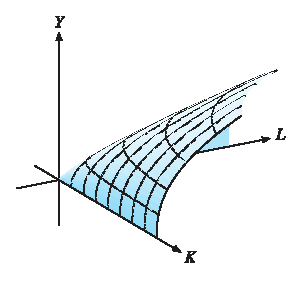
\includegraphics[width=\linewidth]{figure1}\label{fig:1}
			\caption{Gráfica de la función de producción Cobb-Douglas.}
		\end{minipage}
		\hfill
		\begin{minipage}[c]{0.4\linewidth}
			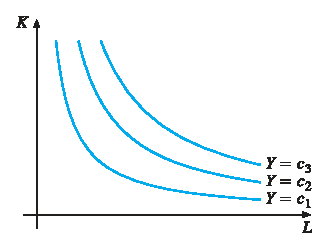
\includegraphics[width=\linewidth]{figure2}\label{fig:2}
			\caption{Isocuantas de la función de producción Cobb-Douglas.}
		\end{minipage}
	\end{figure}
\end{example}
% pag. 428
\begin{example}[Funciones $n$--lineales y $\log$--lineales]
	\leavevmode
	\begin{enumerate}
		\item\label{item:a} La demanda del azúcar en los Estados Unidos durante el período 1929--1936 fue estimado para ser descrito, aproximadamente, por la fórmula \[ x=108.83-6.0294p+0.164w-0.4217t \] donde $x$ es la demanda del azúcar, $p$ es su precio, $w$ es un índice de producción y $t$ es el año (donde $t=0$ corresponde a 1929).
		\item\label{item:b} La siguiente fórmula es una estimación para la demanda de cerveza en el Reino Unido: \[ x=1.058{x}^{0.136}_{1}{x}^{-0.727}_{2}{x}^{0.914}_{3}x^{0.816}_{4}. \]
		Aquí la cantidad demandada, $x$, es una función de cuatro variables: $x_{1}$, el ingreso per cápita, $x_{2}$, el precio de la cerveza, $x_{3}$, índice general de precios de productos básicos y $x_{4}$, la fuerza de la cerveza.
	\end{enumerate}
\end{example}
Las funciones más simples en el ejemplo anterior es la única en la parte~\eqref{item:a}. Las variables $p$, $w$ y $t$ ocurren solo cuando a la primera potencia, y ellas son multiplicadas por constantes, no por cada otra. Tales funciones son llamadas \emph{lineales}. En general
\begin{equation}
f\left(x_{1},x_{2},\ldots,x_{n}\right)=a_{1}x_{1}+a_{2}x_{2}+\cdots+a_{n}x_{n}+b
\end{equation}
donde $a_{1},a_{2},\ldots,a_{n}$ y $b$ son constantes, es una \emph{función lineal} en $n$ variables.

La función en la parte~\eqref{item:b} del ejemplo  es un caso especial de la función general de Cobb-Douglas
\begin{equation}\label{eq:cobbgeneralized}
F\left(x_{1},x_{2},\ldots,x_{3}\right)=A{x}^{a_{1}}_{1}{x}^{a_{2}}_{2}\cdots{x}^{a_{n}}_{n}
\end{equation}
donde $A>0$, $a_{1},\ldots,a_{n}$ son constantes, definidas para $x_{1}>0,x_{2}>0,\ldots x_{n}>0$. Note que al tomar el logaritmo natural a cada lado de~\eqref{eq:cobbgeneralized} resulta
\begin{equation}
\ln F=\ln A+a_{1}\ln x_{1}+a_{2}\ln x_{2}+\cdots+a_{n}\ln x_{n}.
\end{equation}
Esto muestra que la función de Cobb-Douglas es $\log$--lineal, ya que $\ln F$ es una función lineal para $\ln x_{1},\ln x_{2},\ldots,\ln x_{n}$.
\subsection{Modelo de crecimiento de Solow}
\begin{example}[Modelo de crecimiento de Solow]
Este modelo de crecimiento neoclásico está basado en la ecuación diferencial
\begin{equation}\label{eq:solowgrowth}
\dot{k}=sf\left(k\right)-\lambda k
\end{equation}
Aquí la función desconocida $k=k(t)$ denota el capital por trabajador, $s>0$ denota la tasa constante de ahorro, $f$ es una función de producción (producto nacional por trabajador como una función del capital por trabajador), y $\lambda>0$ denota la tasa proporcional constante de crecimiento del número de trabajadores.
\end{example}

Note que~\eqref{eq:solowgrowth} es una ecuacion separable. Debido a que $f$ no se especifica, aún no podemos encontrar una solución explícita de la ecuación. Asuma que el diagrama de fase para la ecuación~\eqref{eq:solowgrowth} es como se muestra en la Fig.4. % TODO: Incluir figura 4.
Luego, aquí un estado de equilibrio único con $k^{\ast}>0$. Esto es dado por:
\begin{equation}
sf\left(k^{\ast}\right)=\lambda k^{\ast}
\end{equation}
Por inspección de la Fig.4 vemos que $k^{\ast}$ es estable. Sin importar cuál ha sido el capital inicial por trabajador $k\left(0\right)$, $k\left(t\right)\rightarrow k^{\ast}$ cuando $t\rightarrow\infty$.

% (pag. 212)
%\caption{Diagrama de fase para~\eqref{eq:solowgrowth}, con condicion apropiada en $f$.}

Este es ua modelo mas detallado que lleva a la ecuación ~\eqref{eq:solowgrowth}. Sea $X\left(t\right)$ que denota el ingreso nacional, $K\left(t\right)$ el capital, y
$L\left(t\right)$ el número de trabajadores en un país en un tiempo $t$. Asuma que
\begin{multicols}{3}
\begin{itemize}
	\item $X\left(t\right)=F\left(K(t),L(t)\right)$
	\item $\dot{K}\left(t\right)=sX\left(t\right)$
	\item $L\left(t\right)=L_{0}e^{\lambda t}$
\end{itemize}
\end{multicols}
donde $F$ es una función de producción, y $s$ es la tasa de ahorro. Asuma que $F$ es homogénea de grado $1$, así que $F\left(K,L\right)=LF\left(K/L,1\right)$ para todo $K$ y $L$.
Defina $k\left(t\right) =K\left(t\right)/L\left(t\right)=$ capital por trabajador, y $f\left(k\right)=F\left(k,1\right)=F\left(K/L,1\right)=F\left(K,L\right)/L=$ salida por trabajador. Luego,  $\dot{k}/k=\left(d/dt\right)\left(\ln k\right)=\left(d/dt\right)\left(\ln K-\ln L\right)$, y así
\begin{equation}
\frac{\dot{k}}{k}=\frac{\dot{K}}{K}-\dfrac{\dot{L}}{L}=\frac{sF\left(K,L\right)}{K}-\lambda=\frac{sLf\left(k\right)}{K}-\lambda=\frac{sf\left(k\right)}{k}-\lambda
\end{equation}
de la cual~\eqref{eq:solowgrowth} sigue a la vez.

\begin{remark}
	Déjenes discutir brevemente las condciones suficientes para la existencia y unicidad del equilibrio del modelo de Solow. Es usual asumir que $f\left(0\right)=0$, así como que $f^{\prime}\left(k\right)>0$ y $f^{\prime\prime}\left(k\right)<0$ para todo $k>0$. Esto es también común postular las llamadas \emph{condiciones de Inada}, de acuerdo con $f^{\prime}\left(k\right)\rightarrow\infty$ y también $f^{\prime}\left(k\right)\rightarrow0$ cuando $k\rightarrow\infty$.
	
	Para ver por qué estas condiciones son suficientes, defina $G\left(k\right)=sf\left(k\right)-\lambda k$. Entonces, $G^{\prime}\left(k\right)=sf^{\prime}\left(k\right)-\lambda$, y la ecuación~\eqref{eq:solowgrowth} cambia a $\dot{k}=G\left(k\right)$. Los supuestos sobre $f$ implica que $G\left(0\right)=0$, $G^{\prime}\left(k\right)\rightarrow\infty$ cuando $k\rightarrow0$, $G^{\prime}\left(k\right)\rightarrow-\lambda<0$ cuando $k\rightarrow\infty$, y $G^{\prime\prime}\left(k\right)=sf^{\prime\prime}\left(k\right)<0$ para todo $k>0$. Así $G$ tiene un único punto estacionario $\hat{k}>0$ en el cual $G^{\prime}\left(\hat{k}\right)=0$. Obviamente, $G\left(\hat{k}\right)>0$. Pero, $G^{\prime}\left(k\right)<-\frac{1}{2}\lambda<0$ para cualquier $k$ suficientemente grande. Se sigue que $G\left(k\right)\rightarrow-\infty$ cuando $k\rightarrow\infty$, así que existe un único punto $k^{\ast}>0$ con $G\left(k^{\ast}\right)=0$. Adicionalmente, $G^{\prime}\left(k^{\ast}\right)<0$. De acuerdo con % TODO
	esta es una condición suficiente para la estabilidad local asintótica de $k^{\ast}$.
\end{remark}
\nocite{*}
\printbibliography[title={Referencias bibliográficas},heading=bibintoc]

\end{document}
\begin{document}

\section{Introducción}

Este proyecto hace referencia a la función de producción de Cobb-Douglas, siendo este publicado en \cite{Douglas1976} 1928 por \citeauthor{Douglas1976}, quienes realizaron un estudio en el que se modeló el crecimiento de la economía estadounidense. Para este proyecto se desarrollará una aplicación con una base de datos como un caso particular, pero previo a su aplicación, se realizará una posible forma de cómo Charles Cobb y Paul Douglas llegaron a la formulación algebraica de la función. Al finalizar, se comparará la solución exacta de la ecuación con la obtenida por el método de mínimos cuadrados.

\subsection{Función de producción de Cobb-Douglas}

Para el análisis matemático de la función, es necesario describir los factores involucrados en el modelo.

\subsection{Función de producción}

Es la relación entre las cantidades máximas de productos que una empresa puede fabricar mediante el uso de diversas cantidades de insumos. Las múltiples funciones de producción están representadas por la combinación de factores de insumo (tecnología, capital, trabajo entre otros). Una función de producción se expresa como la ecuación~\eqref{eq:production} siguiente:
\begin{equation}\label{eq:production}
P=f(K,L,I)
\end{equation}
donde:
\begin{itemize}
	\item $P$ es la cantidad de producción.
	\item $K,L,I$ son los insumos.
\end{itemize}

\section{El proyecto}

En esta sección explicaré los detalles de mi proyecto y su visión. Espero que esta estructura se mejore considerablemente bajo la guía de mi mentor.

\subsection{Cobb-Douglas y la función de producción ACMS}

Partiendo de la función Cobb-Douglas
\begin{equation}%\label{eq:1}
Y = bL^{k}C^{1-k},
\end{equation}
donde:
\begin{itemize}
	\item $b$ representa el factor total de productividad,
	\item $Y$ la producción total,
	\item $L$ el trabajo,
	\item $C$ el capital.
\end{itemize}
Esta función fue generalizada siendo expresada de la manera siguiente:
\begin{equation}%\label{eq:2}
f = \gamma{x}_{1}^{\alpha_{1}}\cdots x_{n}^{\alpha_{n}},
\end{equation}
donde $\gamma$ es una constante positiva y $\alpha_{1},\ldots,\alpha_{n}$ son constantes no cero.

Se dice que una función de producción $f$ es $d$--homogénea o homogénea de degradación $d$, si:
\begin{equation}%\label{eq:3}
f\left(tx_{1},\ldots,tx_{n}\right) = t^{d}f\left(x_{1},\ldots,x_{n}\right),
\end{equation}
Se mantiene para cada $t\in\mathbb{R}$ en la función previamente definida.

Una función \emph{homogénea de degradación uno} es llamado como \emph{linealmente homogéneo}.

Si $d>1$, la función homogénea mostrará un crecimiento a escala, caso contrario cuando $d<1$ mostrará un decrecimiento a escala.

Arrow, Chenery, Minhas y Solow(ACMS) introdujeron una función de producción de dos factores:
\begin{equation}%\label{eq:4}
Q=F\cdot(aK^r + (1-a)L^r)^{1/r},
\end{equation}
donde:
\begin{itemize}
	\item $Q$ representa el resultado,
	\item $F$ el factor de producción,
	\item $a$ el parámetro compartido,
	\item $k,L$ los factores de producción primario,
	\item $r=\left(s-1\right)/s$ , $s=1/\left(1-r\right)$ como la substitución de elasticidad.
\end{itemize}

La función de producción generalizada de ACMS se define:
\begin{equation}\label{eq:5}
f\left(x\right) = \gamma\sum_{i=1}^{n} ({{a}_{i}^{p}x_{i}^{p}})^{d/p},x=\left(x_{1},\ldots,x_{n}\right)\in D\subset\mathbb{R}_{+}^{n},
\end{equation}
con $a_{1},\ldots,a_{n},\gamma,p\neq0$, donde $d$ es la degradación de homogeneidad.

Cabe resaltar que la \emph{función de producción homotética} tiene la siguiente expresión como una función de producción:
\begin{equation}\label{eq:6}
f(x) = F\left(h(x_1,\ldots,x_n\right),
\end{equation}
donde F es una función estrictamente creciente y $h\left(x_1,\ldots,x_n\right)$ es una función homogénea de cualquier degradación d. La \emph{función de producción homotética} de la forma:
\begin{equation}\label{eq:7}
f\left(x\right) = \gamma\sum_{i=1}^{n} ({{a}_{i}^{p}x_{i}^{p}})^{d/p},\quad(\text{resp.},\quad f(x)=F(x_{1}^{\alpha_1}\cdots x_{n}^{\alpha_n}),
\end{equation}
es llamada \emph{función de producción ACMS generalizada homotética}.

\subsection{Breve descripción}

Si $f$ es una función de dos variables, a menudo dejamos que una letra como $z$ denote el valor de $f$ en el punto $\left(x,y\right)$, así $z=f\left(x,y\right)$. Entonces llamaremos a $x$ e $y$ las \emph{variables independientes}, o los \emph{argumentos} de $f$, mientras que $z$ es llamada la \emph{variable independiente}, porque el valor $z$, en general, depende de los valores $x$ e $y$. El dominio de la función $f$ es entonces el conjunto de todos los posibles pares de variables independientes, mientras que su \emph{rango} es el conjunto de valores correspondientes de la variable dependientes. En economía, $x$ e $y$ son llamadas las variables \emph{exógenas}, mientras que $z$ es la variable \emph{endógena}.

Una función de dos variables que aparecen en muchos modelos económicos es
\begin{equation}\label{eq:cobb-douglas}
F\left(x,y\right)=Ax^{a}y^{b}
\end{equation}
donde $A$, $a$ y $b$ son constantes. Usualmente, uno asume que $F$ es definida solo para $x>0$ e $y>0$.

A función de la forma~\eqref{eq:cobb-douglas} es generalmente llamada la \emph{función de Coubb-Douglas}. Se usa con mayor frecuencia para describir ciertos procesos de producción. Entonces $x$ e $y$ son llamados \emph{factores de entrada}, mientras que $F\left(x,y\right)$ es el número de unidades producidas, o la \emph{salida}. En este caso $F$ es llamada la \emph{función de producción}.

%\subsubsection{Defining \pygment{python}{ImageSet} Union for Trigonometric Equation Solver}%\protect||

% TODO: Page 276.
\begin{example}[Elasticidad de sustitución constante]
	Considere la ``elasticidad de sustitución constante'', o la función \textsc{CES}
	\begin{equation}
	F\left(K,L\right)=A\left(aK^{-\rho}+\left(1-a\right)L^{-\rho}\right)^{-1/\rho}
	\end{equation}
	donde $A>0$, $K>0$, $L>0$, $a\in\left(0,1\right)$, y $\rho\neq 0$. Manteniendo $A,K,L$ y $a$ fijos, aplique la regla de L'H\^{o}pital a $z=\ln\left[F\left(K,L\right)/A\right]$  cuando $\rho\to0$ con el fin de mostrar que $F\left(K,L\right)$ converge a la función de Cobb-Douglas $AK^{a}L^{1-a}$.
\end{example}

\begin{proof}[Solución]
	Obtenemos \[ z=\ln{\left(aK^{-\rho}+\left(1-a\right)L^{-\rho}\right)}^{-1/\rho}=-\ln\left(aK^{-\rho}+\left(1-a\right)L^{-\rho}\right)/\rho\to\frac{0}{0}\text{ cuando }\rho\to0. \] Ya que $\left(\mathrm{d}/\mathrm{d}\rho\right)K^{-\rho}=-K^{-\rho}\ln K$ y $\left(\mathrm{d}/\mathrm{d}\rho\right)L^{-\rho}=-L^{-\rho}\ln L$, aplicando la regla de L'H\^{o}pital da
	\begin{align*}
	\lim_{\rho\to0}z
	&=\lim_{\rho\to0}\left[\frac{aK^{-\rho}\ln K + \left(1-a\right)L^{-\rho}\ln L}{aK^{-\rho}+\left(1-a\right)L^{-\rho}}\right]\\
	&=a\ln K+\left(1-a\right)\ln L\\
	&=\ln K^{a}L^{1-a}.
	\end{align*}
	Por lo tanto, $e^{z}\to K^{a}L^{1-a}$. De la definición de $z$, se sigue que $F\left(K,L\right)\to AK^{a}L^{1-a}$ cuando $\rho\to0$.
\end{proof}

%pag. 408-409
\begin{example}[Función de Cobb-Douglas]
	Una función de dos variables que aparece en muchos modelos económicos es
	\begin{equation}\label{eq:cobb}
	F\left(x,y\right)=Ax^{a}y^{b}
	\end{equation}
	donde $A$, $a$ y $b$b son constantes. Usualmente, uno asume que $F$ está definida sola pora $x>0$ e $y>0$.

	Una función $F$ de la forma~\eqref{eq:cobb} es generalmente llamada la \emph{función de Cobb-Douglas}\footnote{La función en~\eqref{eq:cobb} es llamada en honor a los investigadores americanos C.W.Cobb y P.H.Douglas, quien aplicaron esto, con  $a+b=1$, en un articulo científico que aparecio en 1927 en la estimacion de una función de producción. Sin embargo, deberia correctamente ser llamada la ``función de Wicksell'', porque el economista sueco K.Wicksell(1851-1926) introdujo tales funciones de producción antes de 1900.}. Con frecuencia es usada para describir ciertos procesos productivos. Así, $x$ e $y$ son llamados los \emph{factores de entrada}, mientras que $F\left(x,y\right)$ es el número de unidades producidas, o la \emph{salida}. En este caso, $F$ es llamada una \emph{función de producción}.
\end{example}

\begin{example}
	Suponga que $F\left(K,L\right)$ modela la producción de una empresa cuando sus entradas son capital y labor, respectivamente $K$ y $L$. Una curva de nivel por esta función de producción es una curva en el plano $KL$ dado por $F\left(K,L\right)=Y_{o}$, donde $Y_{0}$ es una constante. Esta curva es llamada una \emph{isocuanta}, que significa ``igual cantidad''. Para una función de Cobb-Douglas, $F\left(K,L\right)=AK^{a}L^{b}$, con $a+b<1$ y $A>0$, las figuras~\ref{fig:1} y~\ref{fig:2}, respectivamente, muestra una parte de la gráfica cerca del origen, y tres de las isocuantas.
	
	\begin{figure}[ht!]
		\begin{minipage}[c]{0.4\linewidth}
			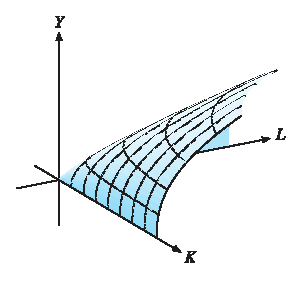
\includegraphics[width=\linewidth]{figure1}\label{fig:1}
			\caption{Gráfica de la función de producción Cobb-Douglas.}
		\end{minipage}
		\hfill
		\begin{minipage}[c]{0.4\linewidth}
			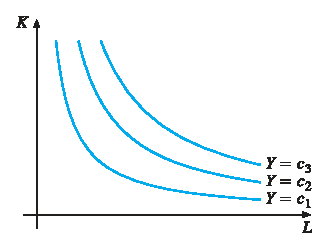
\includegraphics[width=\linewidth]{figure2}\label{fig:2}
			\caption{Isocuantas de la función de producción Cobb-Douglas.}
		\end{minipage}
	\end{figure}
\end{example}
% pag. 428
\begin{example}[Funciones $n$--lineales y $\log$--lineales]
	\leavevmode
	\begin{enumerate}
		\item\label{item:a} La demanda del azúcar en los Estados Unidos durante el período 1929--1936 fue estimado para ser descrito, aproximadamente, por la fórmula \[ x=108.83-6.0294p+0.164w-0.4217t \] donde $x$ es la demanda del azúcar, $p$ es su precio, $w$ es un índice de producción y $t$ es el año (donde $t=0$ corresponde a 1929).
		\item\label{item:b} La siguiente fórmula es una estimación para la demanda de cerveza en el Reino Unido: \[ x=1.058{x}^{0.136}_{1}{x}^{-0.727}_{2}{x}^{0.914}_{3}x^{0.816}_{4}. \]
		Aquí la cantidad demandada, $x$, es una función de cuatro variables: $x_{1}$, el ingreso per cápita, $x_{2}$, el precio de la cerveza, $x_{3}$, índice general de precios de productos básicos y $x_{4}$, la fuerza de la cerveza.
	\end{enumerate}
\end{example}
Las funciones más simples en el ejemplo anterior es la única en la parte~\eqref{item:a}. Las variables $p$, $w$ y $t$ ocurren solo cuando a la primera potencia, y ellas son multiplicadas por constantes, no por cada otra. Tales funciones son llamadas \emph{lineales}. En general
\begin{equation}
f\left(x_{1},x_{2},\ldots,x_{n}\right)=a_{1}x_{1}+a_{2}x_{2}+\cdots+a_{n}x_{n}+b
\end{equation}
donde $a_{1},a_{2},\ldots,a_{n}$ y $b$ son constantes, es una \emph{función lineal} en $n$ variables.

La función en la parte~\eqref{item:b} del ejemplo  es un caso especial de la función general de Cobb-Douglas
\begin{equation}\label{eq:cobbgeneralized}
F\left(x_{1},x_{2},\ldots,x_{3}\right)=A{x}^{a_{1}}_{1}{x}^{a_{2}}_{2}\cdots{x}^{a_{n}}_{n}
\end{equation}
donde $A>0$, $a_{1},\ldots,a_{n}$ son constantes, definidas para $x_{1}>0,x_{2}>0,\ldots x_{n}>0$. Note que al tomar el logaritmo natural a cada lado de~\eqref{eq:cobbgeneralized} resulta
\begin{equation}
\ln F=\ln A+a_{1}\ln x_{1}+a_{2}\ln x_{2}+\cdots+a_{n}\ln x_{n}.
\end{equation}
Esto muestra que la función de Cobb-Douglas es $\log$--lineal, ya que $\ln F$ es una función lineal para $\ln x_{1},\ln x_{2},\ldots,\ln x_{n}$.
\section{Aplicaciones económicas}

\begin{frame}[t]

\begin{theorem}[Igualdad de las derivadas cruzadas o teorema de Schwarz]
Supnga que todas $m$--ésimas derivadas parciales de una función $f\left(x_{1},\ldots,x_{n}\right)$ son continuas. Si cualquiera dos de ellas involucran diferenciación con respecto a cada una de las variables el mismo número de veces, entonces ellas son necesariamente iguales.
\end{theorem}

El contenido de este resultado puede ser explicado como sigue: Sea $m=m_{1}+\cdots+m_{n}$ y suponga que $f\left(x_{1},x_{2},\ldots,x_{n}\right)$ es diferenciable $m_{1}$ veces con respecto a $x_{1}$, $m_{2}$ veces diferenciable con respecto a $x_{2}$, \ldots, y $m_{n}$ veces diferenciable con respecto a $x_{n}$. Suponga que la condición de continuidad es satisfecha por estas derivadas parciales de orden $m$--ésimo. Entonces terminamos con el mismo resultado sin importar cuál sea el orden de la diferenciación, porque cada una de las derivadas parciales es igual a \[ \frac{\partial^{m}f}{\partial x^{m_{1}}_{1}\partial x^{m_{2}}_{2}\cdots\partial x^{m_{n}}_{n}}. \] En particular, para el caso cuando $m=2$, para $i=1,\ldots,n$ y $j=1,\ldots,n$, \[ \frac{\partial^{2}f}{\partial x_{j}\partial x_{i}}=\frac{\partial^{2}f}{\partial x_{i}\partial x_{j}} \] si ambas estas derivadas parciales son continuas.
\end{frame}

\begin{frame}[t]

\begin{example}
Considere la función de producción agricultura $Y=F\left(K,L,T\right)$, donde $Y$ es el número de unidades producidas, $K$ es el capital invertido, $L$ es la entrada trabajo y $T$ es el área de tierra agrícola que es usada. Entonces $\partial Y/\partial K=F^{\prime}_{K}$ es llamada el \emph{capital del producto marginal}. Esta es la tasa de cambio de la salida $Y$ con respecto a $K$ cuando $L$ y $T$ se mantienen fijos. Similarmente, $\partial Y/\partial L=F^{\prime}_{L}$ y $\partial Y/\partial T=F^{\prime}_{T}$ son los productos de trabajo y tierra marginales, respectivamente. Por ejemplo, si $K$ es el valor del capital equipado medido en dólares, y $\partial Y/\partial K=5$, entonces aumentar la entrada de capital en $h$ unidades aumentaría la producción en aproximadamente $5h$ unidades.

Suponga, en particular, que $F$ es la función de Cobb-Douglas $F\left(K,L,T\right)=AK^{a}L^{b}T^{c}$, donde $A$, $a$, $b$ y $c$ son constantes positivas. Encuentre los productos marginales, y las segundas derivadas parciales. Discuta sus signos.
\end{example}

\begin{proof}
Los productos marginales son \[ F^{\prime}_{K}=AaK^{a-1}L^{b}T^{c},\quad F^{\prime}_{L}=AbK^{a}L^{b-1}T^{c},\quad\text{y}\quad F^{\prime}_{T}=AcK^{a}L^{b}T^{c-1}. \] Asumiendo que $K$, $L$ y $T$ son todas positivas, los productos marginales son positivos. Por lo tanto, un incremento en el capital, trabajo o tierra incrementará el número de unidades producidas.

Las segundas derivadas parciales cruzadas, también llamadas parciales mixtas son: \[ F^{\prime\prime}_{KL}=AabK^{a-1}L^{b-1}T^{c},\quad F^{\prime\prime}_{KT}=AacK^{a-1}L^{b}T^{c-1},\quad\text{y}\quad F^{\prime\prime}_{LT}=AbcK^{a}L^{b-1}T^{c-1}. \] Note que estas derivadas son positivas. Llamaremos cada par de factores \emph{complementarios} porque más de uno incrementa el producto marginal de la otra.

Las segunda derivadas parciales directas son \[ F^{\prime\prime}_{KK}=Aa\left(a-1\right)K^{a-2}L^{b}T^{c},\quad F^{\prime\prime}_{LL}=Ab\left(b-1\right)K^{a}L^{b-2}T^{c},\quad F^{\prime\prime}_{TT}=Ac\left(c-1\right)K^{a}L^{b}T^{c-2}. \] Por ejemplo, $F^{\prime\prime}_{KK}$ es la derivada parcial del producto de capital marginal, $F^{\prime}_{K}$ con respecto a $K$. Si $a<1$, entonces $F^{\prime\prime}_{KK}<0$, y existe una disminución del producto del capital marginal, esto es, un pequeño aumento en el capital invertido conducirá a una disminución en el producto marginal del capital Podemos interpretar que esto significa que, aunque pequeños aumentos de capital porque la producción aumentará, así que $F^{\prime}_{K}>0$, este aumento ocurre en una tasa decreciente, dado que $F^{\prime\prime}_{KK}<0$. Similarmente para el trabajo si $b<1$, y para la tierra si $c<1$.
\end{proof}
\end{frame}

\subsection{Elasticidades parciales}

Si $z=f\left(x,y\right)$, definimos la elasticidad parcial de $z$ con respecto a $x$ e $y$ por
\begin{equation}
\operatorname{El}_{x}z=\frac{x}{z}\frac{\partial z}{\partial x},\quad\operatorname{El}_{y}\left(z\right)=\frac{y}{z}\frac{\partial z}{\partial y}
\end{equation}
A menudo los economistas solo se refieren a la elasticidad antes que a la elasticidad parcial. Así, $\operatorname{El}_{x}z$ es la elasticidad de $z$ con respecto a $x$ cuando $y$ se mantiene constante, y $\operatorname{El}_{y}z$ tiene su correspondiente interpretación.

Cuando todas las variables son positivas, las elasticidades pueden expresarse como derivadas logarítmicas. De acuerdo
\begin{equation}
\operatorname{El}_{x}z=\frac{\partial\ln z}{\partial\ln x},\quad\text{y}\quad\operatorname{El}_{y}z=\frac{\partial\ln z}{\partial\ln y}.
\end{equation}

Si $z=f\left(x_{1},x_{2},\ldots,x_{n}\right)=f\left(\bm{x}\right)$, definimos la elasticidad (parcial) de $z$, o de $f$, con respecto a $x_{i}$ como la elasticidad de $z$ con respecto a $x_{i}$ cuando todas las demás variables se mantienen constantes. Así, asumiendo que todas las variables son positivas, podemos escribir
\begin{equation}
\operatorname{El}_{i}z=\frac{x_{i}}{f\left(\bm{x}\right)}\frac{\partial f\left(\bm{x}\right)}{\partial x_{i}}=\frac{x_{i}}{z}\frac{\partial z}{\partial x_{i}}=\frac{\partial\ln z}{\partial\ln x_{i}}.
\end{equation}
El número $\operatorname{El}_{i}z$ es aproximadamente igual al cambio porcentual en $z$ causado por un $1\%$ de incremento en $x_{i}$, la $i$--ésima variable, manteniendo todas las otras $x_{j}$ constantes. Entre otras formas de notación de uso común en lugar de $\operatorname{El}_{i}z$, mencionamos: $\operatorname{El}_{i}f\left(\bm{x}\right)$, $\operatorname{El}_{x_{i}}z$, $\varepsilon_{i}$, $e_{i}$ y $\hat{z}_{i}$. Este último, por supuesto, se pronuncia ``z sombrero i''.


\begin{example}
Suponga que $D=Ax^{a_{1}}_{1}x^{a_{2}}_{2}\cdots x^{a_{n}}_{n}$ es definido para todos los $x_{1}>0$, $x_{2}>0$,\ldots,$x_{n}>0$, donde $A>0$ y $a_{1},a_{2},\ldots,a_{n}$ son constantes. Encuentre la elasticidad de $D$ con respecto a $x_{i}$, para $i=1,\ldots,n$.
\end{example}

\begin{proof}
Debido a que todos los factores excepto $x^{a_{i}}_{i}$ son constantes, podemos aplicar la ecuación (7.7.3) para obtener el resultado $\operatorname{El}_{i}D=a_{i}$.
\end{proof}

Como un caso especial de este ejemplo, suponga que $D_{i}=Am^{\alpha}p^{-\beta}_{i}p^{\gamma}_{j}$, donde $m$ es el ingreso, $p_{i}$ es el propio precio y  $p_{j}$ es el precio de un bien sustituto. Entonces, $\alpha$ es la elasticidad ingreso de la demanda. Por otra parte, $-\beta$ es la elasticidad de la demanda con respecto a los cambios en sus propios precios $p_{i}$, por eso se llama \emph{elasticidad de precio propio} de la demanda. Sin embargo, debido a que las elasticidades de demanda del precio propio son generalmente negativas, a menudo se describe $\beta$ antes que $-\beta$ como la elasticidad de la demanda a precio propio. Finalmente, $\gamma$ es la elasticidad de la demanda con respecto al precio del sustituto especificado. Por analogía con las derivadas parciales cruzadas, se llama \emph{elasticidad de precio cruzado} de la demanda. Tenga en cuenta que la proporción del ingreso gastado en bienes es \[ \frac{p_{i}D_{i}}{m}=Am^{\alpha-1}p^{1-\beta}_{i}p^{\gamma}_{j}. \] Cuando la elasticidad de ingreso $\alpha<1$, esta proporción es una función de ingreso decreciente. Los economistas describen un producto con esta propiedad como una \emph{necesidad}. Por otro lado, cuando $\alpha>1$, la proporción de ingreso gastado en un producto $i$ aumenta con el ingreso, en cuyo caso los economistas describen el producto $i$ como un lujo.

\begin{remark}
Si $z=f\left(x_{1},\ldots,x_{n}\right)$ es continuamente diferenciable y $x_{i}=g_{i}\left(t_{1},\ldots,t_{m}\right)$, para cada $i=1,2,\ldots,n$ son todas diferenciables, entonces \[ \frac{\partial z}{\partial t_{j}}=\frac{\partial z}{\partial x_{1}}\frac{\partial x_{1}}{\partial t_{j}}+\frac{\partial z}{\partial x_{2}}\frac{\partial x_{2}}{\partial t_{j}}+\cdots+\frac{\partial z}{\partial x_{n}}\frac{\partial x_{n}}{\partial t_{j}} \] para cada $j=1,2,\ldots,m$.
\end{remark}

Un pequeño cambio en una variable básica $t_{j}$ desencadena una reacción en cadena. En primer lugar, cualquier $x_{i}$ depende de $t_{j}$ en general, por lo que cambia cuando $t_{j}$ ha cambiado. Esto afecta a su vez a $z$. La contribución de la derivada total de $z$ con respecto a $t_{j}$ que resulta de los cambios en $x_{i}$ es $\left(\partial z/\partial x_{i}\right)\left(\partial x_{i}/\partial t_{j}\right)$. La fórmula (12.2.3) muestra \[ F^{\prime}_{j}\left(\bm{t}\right)=f^{\prime}_{1}\left(\bm{x}\left(\bm{x}\right)\frac{\partial g_{1}}{\partial t_{j}}\left(\bm{t}\right)+f^{\prime}_{2}\left(\bm{x}\left(\bm{x}\right)\frac{\partial g_{2}}{\partial t_{j}}\left(\bm{t}\right)+\cdots+f^{\prime}_{n}\left(\bm{x}\left(\bm{x}\right)\frac{\partial g_{n}}{\partial t_{j}}\left(\bm{t}\right). \]
\begin{frame}

\begin{example}
Considere la función de producción agrícola $Y=F\left(K,L,T\right)$, donde $Y$ es el tamaño de la cosecha, $K$ es el capital invertido, $L$ es el trabajo y $T$ es la tierra agrícola utilizada para cultivar. Suponga que $K$, $L$ y $ T$ son todas funciones del tiempo, que es denotado por $t$. Entonces de acuerdo con (12.2.3), uno tiene
\end{example}

\begin{example}
Suponga que $K$, $L$ y $T$ son todas funciones del tiempo, que es denotado por $t$. Entonces, de acuerdo con
uno tiene
\[ \dfrac{\mathrm{d}Z}{\mathrm{d}t}=\frac{\partial F}{\partial K}\frac{\mathrm{d}K}{\mathrm{d} t}+\frac{\partial F}{\partial L}\frac{\mathrm{d}L}{\mathrm{d}t}ü\frac{\partial F}{\partial T}\frac{\mathrm{d}T}{\mathrm{d}t}. \] En el caso especial cuando $F$ es la función de Cobb-Douglas $F\left(K,L,T\right)=AK^{a}L^{b}T^{c}$, entonces
\begin{equation}\label{eq:dydt}
\frac{\mathrm{d}Y}{\mathrm{d}t}=aAK^{a-1}L^{b}T^{c}\frac{\mathrm{d}K}{\mathrm{d}t}+bAK^{a}L^{b-1}T^{c}\frac{\mathrm{d}L}{\mathrm{d}t}+cAK^{a}L^{b}T^{c-1}\frac{\mathrm{d}T}{\mathrm{d}t}\notag{*}
\end{equation}
Denotando las derivadas temporales por puntos, y dividiendo cada término en~\eqref{eq:dydt} por $Y=AK^{a}L^{b}T^{c}$, tenemos \[ \frac{\dot{Y}}{Y}=a\frac{\dot{K}}{K}+b\frac{\dot{L}}{L}+c\frac{\dot{T}}{T}. \] La tasa relativa de cambio de la salida es, por lo tanto, la suma ponderada de las tasas relativas del cambio del capital, trabajo y tierra. Los pesos son las respectivas potencias $a$, $b$ y $c$.
\end{example}

\end{frame}

\section{Elasticidad de sustitución}

\begin{frame}[t]

Los economistas con frecuencia están interesados en la pendiente de la recta tangente a la curva de nivel en un punto particular. Frecuentemente, la curva de nivel está inclinada hacia abajo, pero los economistas prefieren una respuesta positiva. Así, podemos cambiar el signo de la pendiente, y usar un nombre especial
\begin{definition}[Tasa marginal de sustitución]
\begin{equation}
R_{yx}=\frac{F^{\prime}_{x}\left(x,y\right)}{F^{\prime}_{y}\left(x,y\right)}
\end{equation}
es conocida como la \emph{tasa marginal de sustitución de} $y$ \emph{por} $x$, abreviadamente como \textsc{MRS}.
\end{definition}

Note que $R_{yx}=-y^{\prime}\aprox-\frac{\Delta y}{\Delta x}$ cuando nos movemos a largo de la curva de nivel $F\left(x,y\right)=c$. Si $\Delta x=-1$ en particular, entonces $R_{yx}\approx\Delta y$. Así, $R_{yx}$ es aproximadamente la cantidad de $y$ podemos agregar por unidad de $x$ removida, si permanecemos en la misma curva de nivel.
\end{frame}

\begin{frame}

\begin{example}
Sea $F\left(K,L\right)=100$ una isocuanta para la función de producción, donde $K$ es la entrada de capital, $L$ es la entrada de trabajo y $100$ es la salida. Vea la figura 12.5.1. En todos los puntos $P$, $Q$ y $R$ se producen $100$ unidades. En $P$ un pequeño capital de entrada y bastante entrada de trabajo son empleados. La pendiente de la isocuanta en $P$ es aproximadamente $-4$, así que el \textsc{MRS} en $P$ es aproximadamente $4$. Esto significa que para cada cuatro unidades de trabajo que se llevan, agregando solo una unidad de capital nos asegurará que la salida permanece en (aproximadamente) $100$ unidades. Siempre que se elijan unidades para que el capital y el trabajo tengan el mismo precio, el capital en $P$ es más ``valioso'' que el trabajo. En $Q$ el \textsc{MRS} es aproximadamente $1$, así que el capital y el trabajo son igualmente ``valiosos''. Finalmente, en $R$, el \textsc{MRS} es aproximadamente $\frac{1}{5}$, así en este punto aproximadamente cinco unidades de capital son requeridos para compensar la pérdida de una unidad de trabajo.
\end{example}

\end{frame}

\begin{frame}[t]
Considere la curva de nivel $F\left(x,y\right)=c$ para la función $F$ de dos variables, como es mostrado en la figura 12.5.2. La \textsc{MRS} varía a lo largo de la curva. En el punto $P$, $R_{yx}$ es un número positivo grande. En $Q$, el número $R_{yx}$ es alrededor $1$, y en $R$ este es alrededor de $0.2$. Cuando nos movemos a lo largo de la curva de nivel desde la izquierda hacia la derecha, $R_{yx}$ será estrictamente decreciente con valores en algún intervalo positivo $I$. Para cada valor de $R_{yx}$ en $I$, existe un punto correspondiente $\left(x,y\right)$ en la curva de nivel $F\left(x,y\right)=c$, así un valor correspondiente de $\frac{y}{x}$. La fracción $\frac{y}{x}$ es por lo tanto una función de $R_{zx}$ y se define la siguiente:

\begin{definition}
Cuando $F\left(x,y\right)=c$, la \emph{elasticidad de sustitución entre} $y$ \emph{y} $x$ es \[ \sigma_{yx}=\operatorname{El}_{R_{yx}}\left(\frac{y}{x}\right). \]
\end{definition}

Así, $\sigma_{xy}$ es la elasticidad de sustitución de la fracción $\frac{y}{x}$ con respecto a la \textsc{MRS}. Más o menos, $\sigma_{yx}$ es el porcentaje de cambio en la fracción $\frac{y}{x}$ cuando nos movemos a lo largo de la curva de nivel $F\left(x,y\right)=c$ lo suficientemente lejos para que $R_{yx}$ incremente en un $1\%$. Note que $\sigma_{yx}$ es simétrico en $x$ e $y$. De hecjo, $R_{xy}=\frac{1}{R_{yx}}$, así que la fórmula logarítmica para elasticidades implica que $\sigma_{xy}=\sigma_{yx}$.
\end{frame}

\begin{frame}[t]

\begin{example}
Calcule la elasticidad de sustitución $\sigma_{KL}$ de la función Cobb-Douglas $F\left(K,L\right)=AK^{a}L^{b}$.
\end{example}

\begin{proof}
La \textsc{MRS} de $K$ para $L$ es \[ R_{KL}=\frac{F^{\prime}_{L}}{F^{\prime}_{K}}=\frac{bAK^{a}L^{b-1}}{aAK^{a-1}L^{b}}=\frac{b}{a}\frac{K}{L}. \] Por lo tanto, $\frac{K}{L}=\left(\frac{a}{b}\right)R_{KL}$. La elasticidad de la última expresión con respecto a $R_{KL}$ es $1$. Así, $\sigma_{KL}=1$ para la función de Cobb-Douglas.
\end{proof}

\end{frame}

\begin{frame}

\begin{example}
Encuentre la elasticidad de sustitución para la función \textsc{CES} \[ F\left(K,L\right)=A{\left(aK^{-\rho}+bL^{-\rho}\right)}^{-\mu/\rho} \] donde $A$, $a$, $b$, $\mu$ y $\rho$ son constantes, $A>0$, $a>0$, $b>0$, $\mu\neq0$, $\rho>-1$ y $\rho\neq0$.
\end{example}

\begin{proof}
Aquí
\begin{align*}
F^{\prime}_{K}&=A{\left(-\frac{\mu}{\rho}\right)\left(aK^{-\rho}+bL^{-\rho}\right)}^{\left(-\frac{\mu}{\rho}\right)-1}a\left(-\rho\right)K^{-\rho-1},\\
F^{\prime}_{L}&=A{\left(-\frac{\mu}{\rho}\right)\left(aK^{-\rho}+bL^{-\rho}\right)}^{\left(-\frac{\mu}{\rho}\right)-1}b\left(-\rho\right)L^{-\rho-1}.
\end{align*}
Así, \[ R_{KL}=\frac{F^{\prime}_{L}}{F^{\prime}_{K}}=\frac{b}{a}\frac{L^{-\rho-1}}{K^{-\rho-1}}=\frac{b}{a}{\left(\frac{K}{L}\right)}^{\rho+1} \] y por lo tanto \[ \frac{K}{L}={\left(\frac{a}{b}\right)}^{\frac{1}{\left(\rho+1\right)}}{\left(R_{KL}\right)}^{^{\frac{1}{\left(\rho+1\right)}}} \] Recordando que la elasticidad de $Ax^{b}$ con respecto a $x$ es $b$, implica que \[ \sigma_{KL}=\operatorname{El}_{R_{KL}}\left(\frac{K}{L}\right)=\frac{1}{\rho+1}. \] Hemos mostrado que la función $F$ tiene elasticidad de sustitución constante $\frac{1}{\left(\rho+1\right)}$. Este, por supuesto, es la razón porqué $F$ es llamada la función \textsc{CES} ``elasticidad de sustitución constante''.

Note que la elasticidad de sustitución para la función \textsc{CES} tiende a $1$ cuando $\rho\to0$, el cual es precisamente la elasticidad de sustitución para la función Cobb-Douglas en el ejemplo anterior.
\end{proof}

\end{frame}

\begin{frame}
\begin{definition}
Una función $f$ de dos variables $x$ e $y$ son definidas en un dominio $D$ se dice que es \emph{homogénea de grado} $k$ si, para cualquier $\left(x,y\right)$ en $D$, \[ f\left(tx,ty\right)=t^{k}f\left(x,y\right) \] para cualquier $t>0$. En otras palabras, esto significa que multiplicando ambas variables por un factor positivo $t$ multiplicaremos el valor de la función por el factor $t^{k}$.
\end{definition}
El grado de homogeneidad de una función puede ser un número arbitrario, positivo, cero o negativo. Anteriormente, determinamos el grado de homogeneidad para varias funciones particulares.

Un polinomio es homogéneo de grado $k$ si y solo si la suma de sus exponentes en cada término es $k$. Otros tipos de polinomios con diferentes sumas de exponentes en diferentes términos, tales como $f\left(x.y\right)=1+xy$ o $g\left(x,y\right)=x^{3}+xy$ no son homogéneas de cualquier grado.
\end{frame}


\begin{frame}
La función $f\left(x,y\right)$ es homogénea de grado $k$ si y solo si
\begin{equation}
xf^{\prime}_{1}\left(x,y\right)+yf^{\prime}_{2}\left(x,y\right)=kf\left(x,y\right)
\end{equation}
Esta es una fácil demostración que la ecuación (12.6.2) debe mantenerse cuando $f$ es homogénea de grado $k$:

Diferenciando cada lado de la ecuación (12.6.1) con respecto a $t$, usando la regla de la cadena para diferenciar el lado izquierdo de la ecuación. El resultado es \[ xf^{\prime}_{1}\left(tx,ty\right)+yf^{\prime}_{2}\left(tx,ty\right)=kt^{k-1}f\left(x,y\right). \] Haciendo $t=1$ se obtiene $xf^{\prime}_{1}\left(x,y\right)+yf^{\prime}_{2}\left(x,y\right)=kf\left(x,y\right)$ inmediatamente.
\end{frame}

Notemos otras tres interesantes propiedades generales de funciones $f\left(x,y\right)$ que son homogéneas de grado $k$:
\begin{equation}
f^{\prime}_{1}\left(x,y\right)\text{ y }f^{\prime}_{2}\left(x,y\right)\text{ son ambas homogéneas de grado }k-1
\end{equation}
\begin{equation}
f\left(x,y\right)=x^{k}f\left(1,\frac{y}{x}\right)=y^{k}f\left(\frac{x}{y},1\right)\text{ puesto que }x>0\text{ y }y>0
\end{equation}
y
\begin{equation}
x^{2}f^{\prime\prime}_{11}\left(x,y\right)+2xyf^{\prime\prime}_{12}\left(x,y\right)+y^{2}f^{\prime\prime}_{22}\left(x,y\right)=k\left(k-1\right)f\left(x,y\right)
\end{equation}
Nuevamente, estos resultados no son difíciles de probar:

Para probar (12.6.3), mantenga $t$ e $y$ constantes y diferencia parcialmente con respecto a $x$ la ecuación (12.6.1). Luego, $tf^{\prime}_{1}\left(tx,ty\right)=t^{k}f^{\prime}_{1}\left(x,y\right)$, así $f^{\prime}_{1}\left(tx,ty\right)=t^{k-1}f^{\prime}_{1}\left(x,y\right)$, en consecuencia mostramos que $f^{\prime}_{1}\left(x,y\right)$ es homogénea de grado $k-1$. El mismo argumento muestra que $f^{\prime}_{2}\left(x,y\right)$ es homogénea de grado $k-1$. Uno puede probar que las desigualdades en (12.6.4) al reemplazar $t$ en (12.6.1) primero por $\frac{1}{x}$ y luego por $\frac{1}{y}$, respectivamente. Finalmente, para mostrar (12.6.5), asuma que $f\left(x,y\right)$ es dos veces continuamente diferenciable, notemos primero que debido a $f^{\prime}_{1}\left(x,y\right)$ y $f^{\prime}_{2}\left(x,y\right)$ son ambas homogéneas de grado $k-1$, por el teorema de Euler, podemos aplicar separadamente a $f^{\prime}_{1}$ y luego a $f^{\prime}_{2}$. Esto implica que
\begin{align}
xf^{\prime\prime}_{11}\left(x,y\right)+yf^{\prime\prime}_{12}\left(x,y\right)&=\left(k-1\right)f^{\prime}_{1}\left(x,y\right)\\
xf^{\prime\prime}_{21}\left(x,y\right)+yf^{\prime\prime}_{22}\left(x,y\right)&=\left(k-1\right)f^{\prime}_{2}\left(x,y\right).
\end{align}

Déjenos ahora multiplicar la primera de estas ecuaciones por $x$, la segunda por $y$, y luego sumarlas. Debido a que $f$ es $C^{2}$, por el teorema de Schwarz implica que $f^{\prime\prime}_{12}=f^{\prime\prime}_{21}$, entonces el resultado es \[ x^{2}f^{\prime\prime}_{11}\left(x,y\right)+2xyf^{\prime\prime}_{12}\left(x,y\right)+y^{2}f^{\prime\prime}_{22}\left(x,y\right)=\left(k-1\right)\left[xf^{\prime}_{1}\left(x,y\right)+yf^{\prime}_{2}\left(x,y\right)\right]. \] Por el teorema de Euler, sin embargo, $xf^{\prime}_{1}\left(x,y\right)+yf^{\prime}_{2}\left(x,y\right)=kf\left(x,y\right)$, así (12.6.5) es verificado.

\begin{example}
Suponga que la función de producción $Y=F\left(K,L\right)$ es homogénea de grado $1$. Muestra que uno puede expresar el cociente salida--trabajo $\frac{Y}{L}$ como una función $\frac{Y}{L}=f\left(\frac{K}{L}\right)$ del cociente capital--trabajo $k=\frac{K}{L}$, donde $f\left(k\right)=F\left(k,1\right)$. Encuentre la forma de $f$ cuando $F$ es la función de Cobb-Douglas, con $a+b=1$.
\end{example}

\begin{proof}
Debido a que $F$ es homogénea de grado $1$, es un caso especial de (12.6.4) uno tiene \[ Y=F\left(K,L\right)=F\left(L\left(\frac{K}{L}\right),L\cdot1\right)=LF\left(k,1\right)=Lf\left(k\right) \text{ donde }k=\frac{K}{L}. \] Cuando $F\left(K,L\right)=AK^{a}L^{1-a}$, entonces $f\left(k\right)=F\left\left(k,1\right)=Ak^{a}$.
\end{proof}

\subsection{Aspectos geométricos de las funciones homogéneas}
Las funciones homogéneas en dos variables tienen algunas propiedades geométricas interesantes. Sea $f\left(x,y\right)$ una función homogénea de grado $k$. Considere un rayo en el plano $xy$ desde el origen pasando por el punto $\left(x_{0},y_{0}\right)\neq\left(0,0\right)$. Un punto arbitrario en este rayo es de la forma $\left(tx_{0},ty_{0}\right)$ para algún número positivo $t$. Si dejamos $f\left(x_{0},y_{0}\right)=c$, entonces $f\left(tx_{0},ty_{0}\right)=t^{k}f\left(x_{0},y_{0}\right)=t^{k}c$. Por encima de cualquier rayo en el plano $xy$ pasando por el punto $\left(x_{0},y_{0}\right)$, la porción relativa a la gráfica de $f$ por lo tanto consiste de la curva $z=t^{k}c$, donde $t$ mide la distancia a lo largo del rayo desde el origen, y $c=f\left(x_{0},y_{0}\right)$. Una función que es homogénea de grado $k$ está completamente determinada si su valor es conocido en un punto sobre cada rayo pasando el origen, como en la figura 12.6.1.

En particular, sea $k=1$, así que $f\left(x,y\right)$ es homogénea de grado $1$. La curva $z=t^{k}c$ acostada verticalmente hacia arriba sobre cada rayo que pasa por el origen, es entonces la recta $z=tc$. Debido a esto, a menudo se dice que el \emph{gráfico de una función homogénea de grado} $1$ es generado por rectas que pasan por el origen. La figura 12.6.2 ilustra esto.

Hemos visto cómo, para una función $f\left(x,y\right)$ de dos variables, es a menudo conveniente considerar sus curvas de nivel en el plano $xy$ en vez de su gráfica tridimensional. ¿Qué podemos decir sobre las curvas de nivel de una función homogénea? Resulta que \emph{para una función homogénea, incluso si solo se conoce sus curvas de nivel, también lo son sus otras curvas de nivel}. Para ver esto, considere una función $f\left(x,y\right)$ que es homogénea de grado $k$, y sea $f\left(x,y\right)=c$ una de sus curvas de nivel, como se ilustra en la figura 12.6.3 Ahora explicamos cómo construir la curva de nivel que pasa un por un punto arbitrario $A$ no acostado en $f\left(x,y\right)=c$ en un punto $D$ con coordenadas $\left(x_{1},y_{1}\right)$. Las coordenadas de $A$ tendrán la forma $\left(tx_{1},ty_{1}\right)$ para algún valor de $t$ que en la giura es alrededor de $1.7$.

Con el fin de construir un nuevo punto en la misma curva de nivel como $A$, dibuje un nuevo rayo pasando por el origen. Suponga que este rayo intersecta la curva de nivel original $f\left(x,y\right)=c$ en $\left(x_{2},y_{2}\right)$. Ahora use el valor de $t$ encontrado antes para determinar el nuevo punto $B$ con coordenadas $\left(tx_{2},ty_{2}\right)$. Ahora este nuevo punto $B$ en la misma curva de nivel como $A$ debido a que $f\left(tx_{2},ty_{2}\right)=t^{k}f\left(x_{2},y_{2}\right)=t^{k}c=t^{k}f\left(x_{1},y_{1}\right)=f\left(tx_{1},ty_{1}\right)$. Repitiendo esta construcción para diferentes rayos a través del origen que intersecta la curva de nivel $f\left(x,y\right)=c$, podemos encontrar tantos punto como deseemos en la nueva curva de nivel $f\left(x,y\right)=f\left(tx_{1},ty_{1}\right)$.

El procedimiento argumentado muestra que una función homogénea $f\left(x,y\right)$ está completamente determinada por cualquiera de sus curvas de nivel y por su grado de homogeneidad. La forma de cada curva de nivel de una función homogénea es con frecuencia determinado especificando sus elasticidades de sustitución.

Otro punto que vale la pena notar en relación con la figura 12.6.3 es que las tangentes a las curvas de nivel a lo largo de cada rayo son paralelas. Mantenemos el supuesto que $f$ es homogénea de grado $k$. Si la curva de nivel es $f\left(x,y\right)=c$, su pendiente en el punto $\left(x,y\right)$ es $-f^{\prime}_{1}\left(x,y\right)/f^{\prime}_{2}\left(x,y\right)$. En el punto $A$ en la figura 12.6.3 la pendiente es
\begin{equation}
-\frac{f^{\prime}_{1}\left(tx_{1},ty_{1}\right)}{f^{\prime}_{2}\left(tx_{1},ty_{1}\right)}=-\frac{t^{k-1}f^{\prime}_{1}\left(x_{1},y_{1}\right)}{t^{k-1}f^{\prime}_{2}\left(x_{1},y_{1}\right)}=-\frac{f^{\prime}_{1}\left(x_{1},y_{1}\right)}{f^{\prime}_{2}\left(x_{1},y_{1}\right)}\notag{*}
\end{equation}
donde hemos usado la ecuación (12.6.3), expresando el hecho que las derivadas parciales de $f$ son homogéneas de grado $k-1$. Las igualdades en (*) establecen que dos curvas de nivel pasando por $A$ y $D$ tiene las mismas pendientes en esos puntos. Se sigue que, en cualquier punto a largo de un rayo pasando por el origen, la pendiente de la curva de nivel correspondiente muestra que es la misma. Declarado de manera diferente, después de quitar los signos menos, (*) muestra que la tasa marginal de sustitución de $y$ por $x$ es una función homogénea de grado $0$.

\subsection{Funciones homogéneas y homotéticas}

Suponga que $f$ es una función de $n$ variables definida en su domino $D$. El conjunto $D$ es llamado un \emph{cono} si, cuando $\left(x_{1},x_{2},\ldots,x_{n}\right)\in D$ y $t>0$, el punto $\left(tx_{1},tx_{2},\ldots,tx_{n}\right)$ también se encuentra en $D$. Cuando $D$ es un cono, diremos que la función $f$ es \emph{homogénea de grado} $k$ \emph{en} $D$ si
\begin{equation}
f\left(tx_{1},tx_{2},\ldots,tx_{n}\right)=t^{k}f\left(x_{1},x_{2},\ldots,x_{n}\right)
\end{equation}
para todo $t>0$. La constante $k$ puede ser cualquier número real, positivo, cero o negativo.

\begin{frame}
\begin{definition}
Sea $f$ una función de $n$ variables $\bm{x}=\left(x_{1},\ldots,x_{n}\right)$ definida en un cono $K$. Entonces, $f$ es llamada \emph{homotética} si \[ \forall\bm{x},\bm{y}\in K,f\left(\bm{x}\right)=f\left(\bm{y}\right),t>0\implies f\left(t\bm{x}\right)=f\left(t\bm{y}\right). \]
\end{definition}
\end{frame}

\begin{theorem}
Suponga que $f$ es una función diferenciable de $n$ variables, definida en un cono abierto $D$. Entonces, $f$ es homogénea de grado $k$ si, y solo si, la siguiente ecuación se cumple para todo $\bm{x}$ en $D$:
\begin{equation}
\sum_{i=1}^{n}x_{i}f^{\prime}_{i}\left(\bm{x}\right)=kf\left(\bm{x}\right)
\end{equation}
\end{theorem}
La prueba de este resultado no es difícil, y complementa el argumento dado por el teorema 12.6.1:

\begin{proof}
Suponga que $f$ es homogénea de grado $k$, así satisface la ecuación (12.7.1). Diferenciando esta ecuación con respecto a $t$, cuando $\bm{x}$ es fijado, resulta \[ \sum_{i=1}^{n}x_{i}f^{\prime}_{i}\left(t\bm{x}\right)=kt^{k-1}f\left(\bm{x}\right). \] Haciendo $t=1$ da (12.7.2) inmediatamente.
\end{proof}

Para probar la recíprica, asuma que la ecuación (12.7.2) es válida para cualquier $\bm{x}$ en el cono $D$. Mantenga $\bm{x}$ fijado y defina la función $g$ para todo $t>0$ por $g\left(t\right)=t^{-k}f\left(t\bm{x}\right)-f\left(\bm{x}\right)$. Entonces, diferenciando da
\begin{equation}
g^{\prime}\left(t\right)=-kt^{-k-1}f\left(t\bm{x}\right)+t^{-k}\sum_{i=1}^{n}x_{i}f^{\prime}_{i}\left(t\bm{x}\right).
\end{equation}
Debido a que $t\bm{x}$ se encuentra en $D$, la ecuación (12.7.2) también debe ser válida cuando cada $x_{i}$ es reemplazada por $tx_{i}$. Se sigue que $\sum_{i=1}^{n}\left(tx_{i}\right)f^{\prime}_{i}\left(t\bm{x}\right)=kf\left(t\bm{x}\right)$. Multiplicando esta ecuación por $t^{-k-1}$ y usando esto para sustituir por el último término de (*) implica que, para cualquier $t>0$, uno tiene \[ g^{\prime}\left(t\right)=-kt^{-k-1}f\left(t\bm{x}\right)+t^{-k-1}kf\left(t\bm{x}\right)=0. \] Se sigue que $g\left(t\right)$ debe ser una constante $C$. Obviamente, $g\left(1\right)=0$, así que $C=0$, lo que implica que $g\left(t\right)=0$ para todo $t>0$. De acuerdo con la definición de $g$, esto prueba que $f\left(t\bm{x}=t^{k}f\left(\bm{x}\right)$, así que $f$ en realidad es homogénea de grado $k$.

Una versión interesante de la ecuación de Euler, ecuación (12.7.2) % Pag 488
\subsection{Modelo de crecimiento de Solow}
\begin{example}[Modelo de crecimiento de Solow]
Este modelo de crecimiento neoclásico está basado en la ecuación diferencial
\begin{equation}\label{eq:solowgrowth}
\dot{k}=sf\left(k\right)-\lambda k
\end{equation}
Aquí la función desconocida $k=k(t)$ denota el capital por trabajador, $s>0$ denota la tasa constante de ahorro, $f$ es una función de producción (producto nacional por trabajador como una función del capital por trabajador), y $\lambda>0$ denota la tasa proporcional constante de crecimiento del número de trabajadores.
\end{example}

Note que~\eqref{eq:solowgrowth} es una ecuacion separable. Debido a que $f$ no se especifica, aún no podemos encontrar una solución explícita de la ecuación. Asuma que el diagrama de fase para la ecuación~\eqref{eq:solowgrowth} es como se muestra en la Fig.4. % TODO: Incluir figura 4.
Luego, aquí un estado de equilibrio único con $k^{\ast}>0$. Esto es dado por:
\begin{equation}
sf\left(k^{\ast}\right)=\lambda k^{\ast}
\end{equation}
Por inspección de la Fig.4 vemos que $k^{\ast}$ es estable. Sin importar cuál ha sido el capital inicial por trabajador $k\left(0\right)$, $k\left(t\right)\rightarrow k^{\ast}$ cuando $t\rightarrow\infty$.

% (pag. 212)
%\caption{Diagrama de fase para~\eqref{eq:solowgrowth}, con condicion apropiada en $f$.}

Este es ua modelo mas detallado que lleva a la ecuación ~\eqref{eq:solowgrowth}. Sea $X\left(t\right)$ que denota el ingreso nacional, $K\left(t\right)$ el capital, y
$L\left(t\right)$ el número de trabajadores en un país en un tiempo $t$. Asuma que
\begin{multicols}{3}
\begin{itemize}
	\item $X\left(t\right)=F\left(K(t),L(t)\right)$
	\item $\dot{K}\left(t\right)=sX\left(t\right)$
	\item $L\left(t\right)=L_{0}e^{\lambda t}$
\end{itemize}
\end{multicols}
donde $F$ es una función de producción, y $s$ es la tasa de ahorro. Asuma que $F$ es homogénea de grado $1$, así que $F\left(K,L\right)=LF\left(K/L,1\right)$ para todo $K$ y $L$.
Defina $k\left(t\right) =K\left(t\right)/L\left(t\right)=$ capital por trabajador, y $f\left(k\right)=F\left(k,1\right)=F\left(K/L,1\right)=F\left(K,L\right)/L=$ salida por trabajador. Luego,  $\dot{k}/k=\left(d/dt\right)\left(\ln k\right)=\left(d/dt\right)\left(\ln K-\ln L\right)$, y así
\begin{equation}
\frac{\dot{k}}{k}=\frac{\dot{K}}{K}-\dfrac{\dot{L}}{L}=\frac{sF\left(K,L\right)}{K}-\lambda=\frac{sLf\left(k\right)}{K}-\lambda=\frac{sf\left(k\right)}{k}-\lambda
\end{equation}
de la cual~\eqref{eq:solowgrowth} sigue a la vez.

\begin{remark}
	Déjenes discutir brevemente las condciones suficientes para la existencia y unicidad del equilibrio del modelo de Solow. Es usual asumir que $f\left(0\right)=0$, así como que $f^{\prime}\left(k\right)>0$ y $f^{\prime\prime}\left(k\right)<0$ para todo $k>0$. Esto es también común postular las llamadas \emph{condiciones de Inada}, de acuerdo con $f^{\prime}\left(k\right)\rightarrow\infty$ y también $f^{\prime}\left(k\right)\rightarrow0$ cuando $k\rightarrow\infty$.
	
	Para ver por qué estas condiciones son suficientes, defina $G\left(k\right)=sf\left(k\right)-\lambda k$. Entonces, $G^{\prime}\left(k\right)=sf^{\prime}\left(k\right)-\lambda$, y la ecuación~\eqref{eq:solowgrowth} cambia a $\dot{k}=G\left(k\right)$. Los supuestos sobre $f$ implica que $G\left(0\right)=0$, $G^{\prime}\left(k\right)\rightarrow\infty$ cuando $k\rightarrow0$, $G^{\prime}\left(k\right)\rightarrow-\lambda<0$ cuando $k\rightarrow\infty$, y $G^{\prime\prime}\left(k\right)=sf^{\prime\prime}\left(k\right)<0$ para todo $k>0$. Así $G$ tiene un único punto estacionario $\hat{k}>0$ en el cual $G^{\prime}\left(\hat{k}\right)=0$. Obviamente, $G\left(\hat{k}\right)>0$. Pero, $G^{\prime}\left(k\right)<-\frac{1}{2}\lambda<0$ para cualquier $k$ suficientemente grande. Se sigue que $G\left(k\right)\rightarrow-\infty$ cuando $k\rightarrow\infty$, así que existe un único punto $k^{\ast}>0$ con $G\left(k^{\ast}\right)=0$. Adicionalmente, $G^{\prime}\left(k^{\ast}\right)<0$. De acuerdo con % TODO
	esta es una condición suficiente para la estabilidad local asintótica de $k^{\ast}$.
\end{remark}
\nocite{*}
\printbibliography[title={Referencias bibliográficas},heading=bibintoc]

\end{document}